\chapter{The \textsc{referenced promethee} method}

The second modification of \textsc{promethee ii} that will be studied in this work is called \textsc{referenced promethee} and has initially been proposed by Doan and De Smet in \cite{RefPII}.

The main idea of this method to avoid the rank reversal phenomenon is to use a fixed set of $p$ reference profiles ($\mathcal{R}$).

Iteratively, each of the alternatives $a_i$ from $A$ is added to $\mathcal{R} $\cite{RefPII}:
\begin{equation}
    \mathcal{R}_i = \mathcal{R} \cup a_i
    \label{eqn:reference_set_union_ai}
\end{equation}
Its score is then computed as its net flow score computed on $\mathcal{R}_i$ \cite{RefPII}:
\begin{equation}
    \phi_{ref}(a_i) = \frac{1}{p}\sum_{r \in \mathcal{R}_i} [\pi(a_i,r) - \pi(r, a_i)]
    \label{eqn:ref_flow}
\end{equation}

This net flow will be called the referenced flow.

It is not necessary to apply the full \textsc{promethee ii} method on $\mathcal{R}_i$ since we are not interested in the net flows obtained by the reference profiles, neither by their pairwise preferences $\pi(r, r^{\prime})$. 
Since the number of reference profiles should be relatively small compared to the number of alternatives, the computational complexity of \textsc{referenced promethee} will be smaller than the one of \textsc{promethee ii}.

Finally, the alternatives are ranked according to their referenced flows.
In this way, their scores only depend on a fixed set of reference profiles and therefore the relative ordering between two alternatives can not be influenced by other alternatives. This leads to the impossibility for rank reversals to happen but comes with the additional cost of having to find a fixed and appropriated set of reference profiles.

As it will be seen, the choice of the reference profiles set is of crucial importance.
This chapter mainly consists in the study of the influence of these sets, and methods to find or build satisfactory ones.

The judgment whether a ranking is appropriate or not given the parameters provided by the decision maker goes beyond the scope of this work.
We will therefore focus on finding sets of reference profiles that produce rankings similar to the ones produced by \textsc{promethee ii}, as it can be assumed, due to the wide usage of this method that its rankings are satisfactory enough.
To do so, the quality of a set of reference profiles will be assessed using as indicator Kendall's rank correlation coefficient between the \textsc{promethee ii} rankings and the \textsc{referenced promethee} ones obtained with this set of references.

During the rest of this chapter, as with \textsc{robust promethee}, rankings obtained with \textsc{referenced promethee} will only be compared to rankings obtained with \textsc{promethee ii} which have been obtained with the same sets of shared parameters ($w_c, f_c(.), \dots$).

Before studying how to build or find satisfactory sets of reference profiles, some characterisations of the method and of references sets will be discussed.

\section{Characteristics of sets of reference profiles}

The following properties of reference profiles sets have already been demonstrated in \cite{RefPII}:
\begin{itemize}
    \item Permutations of the evaluations for a given criterion between different reference profiles do not influence the \textsc{referenced promethee} ranking. This means that we can arbitrarily impose that the references in a set must pairwise dominate each other.
    \item \textsc{referenced promethee} respects the natural dominance relation.
\end{itemize}

In this section, two other characteristics of the method will be investigated.
First, the minimal number of references needed to discriminate all the alternatives will be found.
This quantity will then be used to study if it is possible to reproduce the \textsc{promethee ii} rankings with such small amounts of reference profiles.

\subsection{Number of reference profiles needed to discriminate all the alternatives}

A first question that comes to mind when trying to characterize the sets of reference profiles is how many profiles are needed to discriminate all the alternatives of a decision problem.

Indeed, as the next sections focus on trying to find or build references sets, it seems interesting to at least have a rough idea of a lower bound on the quantity of reference profiles that would be needed.

Instinctively, one could suppose that the quantity of references necessary will grow as the size of $A$ grows.
It can be seen from Table \ref{tbl:referenced_PII_draws} that this is not the case.


\begin{table}[h]
    \centering
    \begin{tabular}{c @{\hskip 0.5cm} l l l l}
        \toprule
         & \multicolumn{4}{c}{\bf $n$} \\
         \cmidrule{2-5}
         \bf $p$ & \bf 10  & \bf 20  &  \bf 40    &  \bf  80  \\
        \midrule
         \bf 2  &   13 &  45 & 196 & 840 \\
         \bf 3  &   11 &  47 & 196 & 886 \\
         \bf 5  &   11 &  53 & 173 & 833 \\
         \bf 10 &   16 &  44 & 195 & 829 \\
         \bf 15 &   11 &  34 & 171 & 814 \\
         \bf 25 &   12 &  59 & 165 & 786 \\
        \bottomrule
    \end{tabular}
    %\captionsetup{width=10cm}
    \caption{Quantity of couples of indifferent alternatives (sum of 60 repetitions from the \textsc{epi}, \textsc{shanghai}, \textsc{geq} data sets with random parameters with an indifference threshold of 0.001) for a set of $n$ alternatives evaluated with $p$ reference profiles.}
    \label{tbl:referenced_PII_draws}
\end{table}


% This table has been build by applying the \textsc{referenced promethee} method on 60 random subsets of the \textsc{epi}, \textsc{geq}\footnote{The Gender EQuality data set makes also part of the \textsc{epi} project} and the \textsc{shanghai} data sets (20 subsets from each). The other parameters have be chosen at random for each subset.
% The reference profiles used where also build randomly but with the constraint that their evaluations, for each criteria, must be in the same range as the data set on which the method is applied.

% Each cell of this table contains the cumulated number of draws for each of the 60 application of the \textsc{referenced promethee} method (a draw being a pair of alternatives whose referenced flow are closer than a chosen threshold of $0.001$).

As expected, the number of draws between the alternatives increases with the quantity of alternatives of the decision problem, but it does not (or at least not significantly) decrease with the quantity of reference profiles used.

It can therefore be concluded that few reference profiles are sufficient to discriminate as well as possible all the alternatives of a problem (with an indifference threshold that should however decrease as the number alternatives increases).

It will now be investigated if \textsc{referenced promethee} can reproduce \textsc{promethee ii} rankings and particularly if this can be done with a small quantity of reference profiles.

\subsection{Possibility of replicating the \textsc{promethee ii} rankings}
\label{sec:genetic_alg}

Before trying to find methods that build references sets that reproduce the \textsc{promethee ii} rankings it should be verified whether such references sets exist or not.
To answer this question, a first solution that came to our mind was to use a genetic algorithm \cite{Whitley1994}. 
% More particularly, a genetic algorithm \cite{Whitley1994} will be used.

A genetic algorithm is an iterative algorithm inspired by the process of natural selection that took and is still taking place during the evolution of life.
These algorithms are usually used to find ``good solutions'' for nonlinear or hard optimisation problems where it is not possible to find an optimal solution in a reasonable amount of time.

Genetic algorithms work as follows.
At each iteration a population of individuals, which is usually called a generation, is considered.
Each of them is evaluated using the objective function provided with the problem.
The individuals of the population are then combined to form a new generation.
This step is called the reproduction.
Only those with the best scores are selected for the reproduction and the higher the score they obtain, the more they will reproduce.
After the reproduction, some random mutations can also occur (with low probability) which should help the algorithm not to get stuck in a local optimum.
There can be different termination conditions for this algorithm. The algorithm can stop after a given number of iterations, after a given amount of elapsed time or when one of the individuals reaches a score judged as sufficient by the user.

A genetic algorithm is particularly well suited for the problem of finding a set of references profiles since:
\begin{itemize}
    \item The score that must be optimized (the Kendall rank correlation coefficient) is not linear with regard to the reference profiles used.
    \item Sets of reference profiles are well suited for the reproduction operation. Two new sets can be obtained by shuffling the reference profiles of two existing ones.
\end{itemize}
A sketch of a general genetic algorithm is illustrated in the Algorithm \ref{alg:genetic_alg}.
\begin{algorithm}[h]
\begin{algorithmic}[1]
    \REQUIRE population\_size, mutation\_probability, $\mathcal{F}$, MAXIT, CEIL
    \STATE population = initial\_popultaion(population\_size)
    \STATE scores = evaluate\_population(population, $\mathcal{F}$)
    \STATE iteration = 0
    \WHILE{max(scores) < CEIL \AND iteration < MAXIT}
        \STATE population\_fitness = compute\_fitness(scores, population\_size)
        \STATE parents = chose\_parents(population\_fitness)
        \STATE population = combine(parents)
        \STATE population = mutate(population, mutation\_probability)
        \STATE scores = evaluate\_population(population, $\mathcal{F}$)
        \STATE iteration = iteration + 1
    \ENDWHILE
    \RETURN population
\end{algorithmic}
\caption{generic genetic algorithm}
\label{alg:genetic_alg}
\end{algorithm}

This algorithm make uses of some ``genetic algorithm specific elements'' which had to be defined for our specific research of optimal references sets:
\begin{description}
    \item[population: ] collection of possible sets of reference profiles (each set being considered as an individual).
    \item[objective function $\mathcal{F}$: ] Kendall's correlation tau between the ranking obtained by the concerned individual and the ranking obtained with \textsc{promethee ii}.  
    \item[evaluate\_population(): ] evaluate each individual of the population using the objective function.
    \item[compute\_fitness(): ] compute the number of times each individual will be parent according to its score.
    \item[combine\_parents(): ] randomly form pairs of parents. The reference profiles of a pair of parents are shuffled and separated to form two new sets of reference profiles which will, after mutation, form the individuals of the next generation.

        One example of combination of two parents formed by four references can be seen in the figure here under.
\begin{figure}[h]
    \begin{center}
    %\begin{tikzpicture}[line cap=round,line join=round,>=triangle 45,x=1.0cm,y=1.0cm]
     \begin{tikzpicture}[scale=1, transform shape, x=0.25cm,y=0.25cm]
\fill[fill=black,fill opacity=0.1] (2,16) -- (6,16) -- (6,15) -- (2,15) -- cycle;
\fill[fill=black,fill opacity=0.1] (2,14) -- (6,14) -- (6,13) -- (2,13) -- cycle;
\fill[fill=black,fill opacity=0.1] (2,17) -- (2,18) -- (6,18) -- (6,17) -- cycle;
\fill[fill=black,fill opacity=0.1] (2,20) -- (2,19) -- (6,19) -- (6,20) -- cycle;
\fill[color=qqzzqq,fill=qqzzqq,fill opacity=0.1] (17,13) -- (21,13) -- (21,14) -- (17,14) -- cycle;
\fill[color=qqzzqq,fill=qqzzqq,fill opacity=0.1] (17,15) -- (21,15) -- (21,16) -- (17,16) -- cycle;
\fill[color=qqzzqq,fill=qqzzqq,fill opacity=0.1] (21,17) -- (21,18) -- (17,18) -- (17,17) -- cycle;
\fill[color=qqzzqq,fill=qqzzqq,fill opacity=0.1] (17,20) -- (17,19) -- (21,19) -- (21,20) -- cycle;
\fill[color=qqzzqq,fill=qqzzqq,fill opacity=0.1] (2,6) -- (6,6) -- (6,5) -- (2,5) -- cycle;
\fill[color=qqzzqq,fill=qqzzqq,fill opacity=0.1] (17,8) -- (17,7) -- (21,7) -- (21,8) -- cycle;
\fill[color=qqzzqq,fill=qqzzqq,fill opacity=0.1] (17,4) -- (21,4) -- (21,3) -- (17,3) -- cycle;
\fill[color=qqzzqq,fill=qqzzqq,fill opacity=0.1] (17,2) -- (21,2) -- (21,1) -- (17,1) -- cycle;
\fill[fill=black,fill opacity=0.1] (2,8) -- (2,7) -- (6,7) -- (6,8) -- cycle;
\fill[fill=black,fill opacity=0.1] (2,4) -- (6,4) -- (6,3) -- (2,3) -- cycle;
\fill[fill=black,fill opacity=0.1] (2,2) -- (6,2) -- (6,1) -- (2,1) -- cycle;
\fill[fill=black,fill opacity=0.1] (17,6) -- (21,6) -- (21,5) -- (17,5) -- cycle;
\draw (0,21)-- (7,21)-- (7,12)-- (0,12);
\draw [color=qqzzqq] (15,21)-- (22,21)-- (22,12)-- (15,12);
\draw [color=qqzzqq] (15,21)-- (15,12);
\draw (0,21)-- (0,12);
\draw [color=ttttff] (0,9)-- (7,9);
\draw [color=ttttff] (7,9)-- (7,0);
\draw [color=ttttff] (7,0)-- (0,0);
\draw [color=ttttff] (0,0)-- (0,9);
\draw [color=ttttff] (15,9)-- (22,9);
\draw [color=ttttff] (22,9)-- (22,0);
\draw [color=ttttff] (22,0)-- (15,0);
\draw [color=ttttff] (15,0)-- (15,9);
\draw (2,16)-- (6,16);
\draw (6,16)-- (6,15);
\draw (6,15)-- (2,15);
\draw (2,15)-- (2,16);
\draw (2,14)-- (6,14);
\draw (6,14)-- (6,13);
\draw (6,13)-- (2,13);
\draw (2,13)-- (2,14);
\draw (2,17)-- (2,18);
\draw (2,18)-- (6,18);
\draw (6,18)-- (6,17);
\draw (6,17)-- (2,17);
\draw (2,20)-- (2,19);
\draw (2,19)-- (6,19);
\draw (6,19)-- (6,20);
\draw (6,20)-- (2,20);
\draw (1,20.46) node[anchor=north] {\small ${r_1}$};
\draw (1,18.46) node[anchor=north] {\small ${r_2}$};
\draw (1,16.46) node[anchor=north ] {\small ${r_3}$};
\draw (1,14.46) node[anchor=north ] {\small ${r_4}$};
% in the children
\draw (1,8.46) node[anchor=north] {\small ${r_1}$};
\draw (16,6.46) node[anchor=north] {\small ${r_2}$};
\draw (1,4.46) node[anchor=north ] {\small ${r_3}$};
\draw (1,2.46) node[anchor=north ] {\small ${r_4}$};
\draw [color=qqzzqq] (17,13)-- (21,13);
\draw [color=qqzzqq] (21,13)-- (21,14);
\draw [color=qqzzqq] (21,14)-- (17,14);
\draw [color=qqzzqq] (17,14)-- (17,13);
\draw [color=qqzzqq] (17,15)-- (21,15);
\draw [color=qqzzqq] (21,15)-- (21,16);
\draw [color=qqzzqq] (21,16)-- (17,16);
\draw [color=qqzzqq] (17,16)-- (17,15);
\draw [color=qqzzqq] (21,17)-- (21,18);
\draw [color=qqzzqq] (21,18)-- (17,18);
\draw [color=qqzzqq] (17,18)-- (17,17);
\draw [color=qqzzqq] (17,17)-- (21,17);
\draw [color=qqzzqq] (17,20)-- (17,19);
\draw [color=qqzzqq] (17,19)-- (21,19);
\draw [color=qqzzqq] (21,19)-- (21,20);
\draw [color=qqzzqq] (21,20)-- (17,20);
\draw [color=qqzzqq] (2,6)-- (6,6);
\draw [color=qqzzqq] (6,6)-- (6,5);
\draw [color=qqzzqq] (6,5)-- (2,5);
\draw [color=qqzzqq] (2,5)-- (2,6);
\draw [color=qqzzqq] (17,8)-- (17,7);
\draw [color=qqzzqq] (17,7)-- (21,7);
\draw [color=qqzzqq] (21,7)-- (21,8);
\draw [color=qqzzqq] (21,8)-- (17,8);
\draw [color=qqzzqq] (17,4)-- (21,4);
\draw [color=qqzzqq] (21,4)-- (21,3);
\draw [color=qqzzqq] (21,3)-- (17,3);
\draw [color=qqzzqq] (17,3)-- (17,4);
\draw [color=qqzzqq] (17,2)-- (21,2);
\draw [color=qqzzqq] (21,2)-- (21,1);
\draw [color=qqzzqq] (21,1)-- (17,1);
\draw [color=qqzzqq] (17,1)-- (17,2);
\draw (2,8)-- (2,7);
\draw (2,7)-- (6,7);
\draw (6,7)-- (6,8);
\draw (6,8)-- (2,8);
\draw (2,4)-- (6,4);
\draw (6,4)-- (6,3);
\draw (6,3)-- (2,3);
\draw (2,3)-- (2,4);
\draw (2,2)-- (6,2);
\draw (6,2)-- (6,1);
\draw (6,1)-- (2,1);
\draw (2,1)-- (2,2);
\draw (17,6)-- (21,6);
\draw (21,6)-- (21,5);
\draw (21,5)-- (17,5);
\draw (17,5)-- (17,6);
%central arrow 
\path[draw=black,solid,line width=0.5mm,fill=black,
preaction={-triangle 90,thin,draw,shorten >=-1mm}
] (11,11.5) -- (11,9.5);
% \draw [line width=1pt] (10.5,10)-- (11.1,9.5);
% \draw [line width=1pt] (11,9.5)-- (11.6,10);
% \draw [line width=1pt] (11,9.5)-- (11,11.5);
\draw (0,23.29) node[anchor=north west] {$Parent_1$};
\draw [color=qqzzqq](15,23.29) node[anchor=north west] {$Parent_2$};
\draw [color=ttttff](16,11.29) node[anchor=north west] {$Child_2$};
\draw [color=ttttff](1,11.29) node[anchor=north west] {$Child_1$};
         \end{tikzpicture}
\caption{Representation of the combination of two sets of reference profiles}
   \end{center}
\end{figure}

    \item[mutate(): ] modify each evaluation, of each reference, in each reference set of the new population with a low probability.
        The modification of an evaluation consist in multiplying it by a factor taken uniformly at random between $0.75$ and $1.25$.
\end{description}

This genetic algorithm has been applied on random subsets of alternatives of different sizes.
The proportion of subsets for which a set of reference profiles which reproduces the \textsc{promethee ii} ranking exactly has been found is summarised in Table \ref{tbl:genetic_results}.

\begin{table}[h]
    \centering
    \begin{tabular}{c l l l l l l l l}
        \toprule
        & & \multicolumn{3}{c}{4 references} &\phantom{abc} & \multicolumn{3}{c}{5 references} \\
        \cmidrule{3-5} \cmidrule{7-9}
        \bf \textit{n} & & \textsc{epi} &  \textsc{sha} & \textsc{geq}& &  \textsc{epi} &  \textsc{sha} & \textsc{geq}  \\
        \midrule
         \bf 20  & &  15/15 &  15/15 & 14/15 & &      &       & 0/1 \\
         \bf 25  & &  14/15 &  13/15 & 14/15 & &  0/1 &  2/2  & 0/1 \\
         \bf 30  & &  15/15 &  12/15 & 12/15 & &      &  3/3  & 3/3 \\
         \bf 40  & &  13/15 &   8/15 &  7/15 & &  0/2 &  3/7  & 1/8 \\
         \bf 50  & &  10/15 &   2/15 &  2/15 & &  1/5 &  4/13 & 5/13 \\
        \bottomrule
    \end{tabular}
    %\captionsetup{width=10cm}
    \caption{Proportion of random subsets reproducing the \textsc{promethee ii} ranking found with the genetic algorithm.}
    \label{tbl:genetic_results}
\end{table}

First, the algorithm has been applied on 45 different data set of each size searching for sets of 4 reference profiles. 
Then, the algorithm has been retried for each of the data set for which no perfect set had been found but searching this time for sets of $5$ reference profiles.

For each of the different configurations shown in this table, the worst correlation coefficient found from all of the 15 random subsets (or from the remaining subsets when 5 reference profiles where used) is indicated in the Table \ref{tbl:genetic_tau}.

\begin{table}[h]
    \centering
    \begin{tabular}{c l l l l l l l l}
        \toprule
        & & \multicolumn{3}{c}{4 references} &\phantom{abc} & \multicolumn{3}{c}{5 references} \\
        \cmidrule{3-5} \cmidrule{7-9}
        \bf \textit{n} & & \textsc{epi} &  \textsc{sha} & \textsc{geq}& &  \textsc{epi} &  \textsc{sha} & \textsc{geq}  \\
        \midrule
         \bf 20  & &  1.0   & 1.0    & 0.989 & &        &       & 0.884 \\
         \bf 25  & &  0.993 & 0.94   & 0.98  & &  0.946 &  1.0  & 0.993 \\
         \bf 30  & &  1.0   & 0.912  & 0.96  & &        &  1.0  &  1.0 \\
         \bf 40  & &  0.964 & 0.828  & 0.899 & &  0.941 &  0.948 & 0.884 \\
         \bf 50  & &  0.88  & 0.905  & 0.841 & &  0.947 &  0.929 & 0.875 \\
        \bottomrule
    \end{tabular}
    %\captionsetup{width=10cm}
    \caption{Worst $\tau_K$ between the \textsc{promethee ii} ranking and \textsc{referenced promethee} rankings with the best set of reference profiles found with the genetic algorithm.}
    \label{tbl:genetic_tau}
\end{table}
\newpage 
For most random subsets of size smaller or equal to 30, it has been possible to find sets of reference profiles that reproduce exactly the \textsc{promethee ii} ranking.
For the few subsets where this was not the case, the best sets of references found by the genetic algorithm however produced rankings relatively similar to the one obtained with \textsc{promethee ii} (the worst correlation coefficient being $0.912$).  

For larger subsets of alternatives, there is a strong decrease in the proportion for which a set of reference profiles which perfectly reproduces the \textsc{promethee ii} ranking has been found. However, the sets found by the algorithm again produce quite similar rankings (the worst correlation coefficient being $0.828$).

It should also not be forgotten that this genetic algorithm is a heuristic, aimed at providing good solutions for hard optimisation problems.
The fact that no perfect set of reference profiles was found in some configurations does not imply that these do not exist.

% It can be concluded from these results that small sets of reference profiles that produces rankings similar enough to the \textsc{promethee ii} ranking seems to always exist.
 From these results we can conclude that there seem to always exist small sets of reference profiles producing rankings similar to the \textsc{promethee ii} rankings.
It is therefore justified to try to build methods and procedures which should provide such sets of references.
This will be done in the next section.

\section{Constructive methods to build sets of reference profiles}

%To be able to use the \textsc{referenced promethee} method and to analyse it, we must also be able to find sets of reference profiles 
\textsc{referenced promethee} is based on the comparison of the alternatives with a set of reference profiles.
Without providing some tools to find some sets of reference profiles to be used, the method becomes practically unusable. 
Therefore, two approaches to produce sets of reference profiles will be analysed.

The first approach that will be studied relies on defining a construction strategy that builds sets of reference profiles given the sets of alternatives on which the method is applied.
This approach is relatively simple and does not require much additional information from the decision maker.

The second approach, on the other hand, is an interactive approach based on a questioning procedure.
The aim of this procedure is to restrain the set of all possible references sets to only ones producing rankings consistent with the decision maker's answers (under the hypothesis that he answers coherently).

\subsection{Building sets of reference profiles using strategies}
\label{sec:strategies}

When asked to build a set of reference profiles that would be used to apply \textsc{referenced promethee} on a set of alternatives $A$, some obvious possibilities could come to mind.
For example, a possibility could consist in selecting profiles with evaluations which are equally spread from the worst to the best evaluation of the alternatives for each criterion.
Another possibility could consist in using percentiles of the evaluations of the alternatives.

Such ideas will be the basis for what will be called strategies.
An infinite number of different strategies could be considered but only four will be compared in this work. These are presented here under:

\begin{description}
    \item[Strategy I:] build $p$ alternatives at random.
    \item[Strategy II:] build $p$ alternatives as percentiles of the evaluations of $A$.
    \item[Strategy III:] build $p$ alternatives equally spaced between the evaluations of $A$.
    \item[Strategy IV:] build $p$ alternatives as percentiles between the first and the third quartiles of the evaluations of $A$.
\end{description}

These strategies have been used to build sets of references for different random subsets from the three following data sets: \textsc{epi}, \textsc{shanghai} and \textsc{geq} (\textsc{geq} being a particular subset of the \textsc{hdi} project concerning the gender equality conditions in different countries).

Since it has been seen in the previous section that it was generally possible to reproduce the \textsc{promethee ii} ranking with sets of $4$ reference profiles, the simulations in this section, applied on sets of $20$ alternatives, have also been performed with strategies producing $4$ references.

The correlation tau obtained between the \textsc{promethee ii} ranking and the ones produced by \textsc{referenced promethee} used with the specified strategies are shown in Table \ref{tbl:strategies_taus}.
The tests have been performed for 9 subsets ($S$) of alternatives taken uniformly at random.

\begin{table}[h]
    \centering
    \small
    \begin{tabular}{l @{\hskip 2em} c  c c @{\hskip 2em} c c c @{\hskip 2em} c c c}
        \toprule
        &\multicolumn{3}{c@{\hskip 3em}}{\textsc{epi}} &  \multicolumn{3}{c@{\hskip 2em}}{\textsc{sha}}  & \multicolumn{3}{c}{\textsc{geq}}\\
        \cmidrule(r{2em}){2-4} \cmidrule(r{2em}){5-7} \cmidrule(r{0.5em}){8-10}
        \bf \text{Strategy} & $S_1$ & $S_2$ & $S_3$  & $S_4$ &  $S_5$ & $S_6$  & $S_7$  & $S_8$ & $S_9$ \\
        \midrule
        \bf I               & 0.50 & 0.60  & 0.44    &  0.39 &   0.54 &   0.61 &  0.19 &  0.33 &  0.37    \\
        \bf II              & 0.75 & 0.72  & 0.39    &  0.56 &   0.57 &   0.92 &  0.63 &  0.58 &  0.21    \\
        \bf III             & 0.43 & 0.45  & 0.14    &  0.48 &   0.42 &   0.24 &  0.50 &  0.23 &  0.16    \\
        \bf IV              & 0.80 & 0.46  & 1.0     &  0.45 &   0.79 &    1.0 &  0.59 &  0.57 &  0.64    \\
        \bottomrule
    \end{tabular}
    %\captionsetup{width=10cm}
    \caption{Kendall's correlation coefficients obtained between the \textsc{promethee ii} and \textsc{referenced promethee} rankings for different strategies. ($n=20$)}
    \label{tbl:strategies_taus}
\end{table}

The results seem to show that only strategies II and IV produce rankings more similar to the \textsc{promethee ii} ones than by using sets of random reference profiles (strategy I).
There is, on the other hand, no strategy which performs better than any other on all the random subsets, or even which produces satisfying rankings on all the subsets.

In Table \ref{tbl:tau_estimators}, some statistical estimators of the strategies which have been computed on a larger number of random subsets are shown.

\begin{table}[h]
    \centering
    \begin{tabular}{l l l l l}
        \toprule
        \bf Strategy & & \bf $\tau_{min}$  &  \bf $\mu(\tau)$  &  \bf  $\sigma^2(\tau)$ \\
        \midrule
         \bf I  & &   -0.328 & 0.31 & 0.045  \\
         \bf II & &   -0.222 & 0.49 & 0.051  \\
         \bf III& &   -0.31  & 0.36 & 0.043  \\
         \bf IV & &   -0.029 & 0.69 & 0.038  \\
        \bottomrule
    \end{tabular}
    %\captionsetup{width=10cm}
    \caption{Statistical estimators of Kendall's correlation tau for 3000 randoms subsets of 20 alternatives (from the \textsc{epi}, \textsc{shanghai} and \textsc{geq} data sets)}
    \label{tbl:tau_estimators}
\end{table}

From these new results it can be confirmed that no strategy is guaranteed to produce similar ranking to \textsc{promethee ii} rankings. Each strategy produced at least one ranking with a negative correlation coefficient for one of the subsets.
However, the rankings produced by the fourth strategy have an average coefficient of nearly $0.7$.

As the strategies proposed in this section do not produce satisfying enough results, a more elaborated procedure for building sets of reference profiles will be detailed in the next section.
This new procedure should provide references sets that produce rankings more similar to the \textsc{promethee ii} ones at the cost of needing more informations from the decision maker.

\subsection{Building sets of reference profiles using an adaptative questioning procedure}
\label{sec:questioning_procedure}

% The procedure developed in this section is a simplified adaptive questioning procedure based on the one presented by Eppe and De Smet in \cite{eppe2014adaptive} with the difference that it will be aimed at finding a set of reference profiles $\mathcal{R}$ instead of vector of weights $w$.
The procedure developed in this section is a simplified adaptive questioning procedure based on the one presented by Eppe and De Smet in \cite{eppe2014adaptive} with the difference that it will not be aimed at finding a vector of weights $w$.
This new procedure is instead aimed at, given a decision problem (a set $A$ of $n$ alternatives evaluated on $k$ criteria) and given a decision maker (preference functions and a vector of weights $w$), finding a set $\mathcal{R}$ of $p$ reference profiles which leads to a ``satisfactory'' \textsc{referenced promethee} ranking.
The resulting questioning procedure would then act as black box to provide such sets to the decision maker.
\newpage
Since we are interested in this work in finding references sets which reproduce the rankings obtained with the \textsc{promethee ii} method, we will consider an artificial decision maker which provides answers consistent with these rankings.
% Since we are trying to reproduce with the \textsc{referenced promethee} method the rankings produced with \textsc{promethee ii}, it will be supposed that the decision maker.

% In the rest of this section, the adaptive questioning algorithm used will be presented and compared with the one presented in \cite{eppe2014adaptive}, then some results of the application of the algorithm will be discussed.

In the rest of this section, a simplification of the original adaptive questioning procedure presented in \cite{eppe2014adaptive} will first be described, then the modifications that were needed to apply this method for searching sets of reference profiles will be detailed.
Finally, some results of the application of the new method will be discussed.

\subsubsection{Adaptive questioning procedure defining a vector of weights}

Here under a synthesis of the procedure presented in \cite{eppe2014adaptive} is given.

The procedure consists in the delimitation, in a $k$ dimensional space, of a domain $\Omega$ representing the possible values of the vector of weight $w$. \\
Each point $\alpha$ of this domain thus represents a valid weight vector $w_{\alpha}$ and can be associated to the ranking obtained by applying \textsc{promethee ii} with $w_{\alpha}$.
% Each point $\alpha$ of this domain therefore represent a valid weight factor $w_{\alpha}$.
% Each of these points can be associated to the ranking that is obtained by applying the \textsc{promethee ii} method with the corresponding vector of weights.
Each domaine $\Omega$ is therefore associated with a set consisting of all the admissible rankings (that will be called $\Gamma$).
Even if the number of points in $\Omega$ is infinite, there can only be a discrete number of rankings and $\Gamma$ will therefore be finite and discrete.

The procedure works as follows.
At each iteration $i$, a query is asked to the decision maker.
Three types of queries where initially proposed by Eppe and De Smet but only one type will be considered here (since this is the only type of query used in the procedure aimed at finding sets of reference profiles).

This type of query consists in proposing two alternatives of $A$ to the decision maker and asking him which of the two he prefers.
% It starts by considering the whole $p \times k$ dimensional space $\Omega_0$ representing the evaluations the $p$ references of all the possible references sets.
% At each iteration $i$, a question is asked to the decision maker.
% The questions consists in proposing him two alternatives from the $A$ and asking him which of the two he prefers.
His answer will yield a constraint on the domain $\Omega$ of possible weight factors, reducing its size.
By denoting $\Omega_i$ the domain still admissible at the iteration $i$:

\begin{equation}
    \Omega_{i+1} \supseteq \Omega_i
\end{equation}

Suppose for example that the decision maker answers that he prefer alternative $a_i$ over alternative $a_j$. This means that $\phi(a_i)$ should be greater than $\phi(a_j)$. 
\newpage
With the introduction of the uni-criterion net flow $\phi_c$, $\phi(a_i)$ can be written as:

\begin{equation}
    \begin{split}
    \phi(a_i) & = \frac{1}{n-1}\sum\limits^n_{x=1}\sum\limits^k_{c=1} w_c \cdot \big(P_c(a_i,a_x) - P_c(a_x, a_i)\big) \\
              & = \sum\limits^k_{c=1} w_c \left[\frac{1}{n-1} \sum\limits^n_{x=1} \big(P_c(a_i,a_x) - P_c(a_x, a_i)\big)\right] \\
              & = \sum\limits^k_{c=1} w_c \ \phi_c(a_i) \\
    \end{split}
\end{equation}

Since all the parameters needed to compute the uni-criterion net flows of any alternative are constant, these will also be constant.

The answer of the decision maker will therefore result in the following constraint on $w$ \cite{eppe2014adaptive}:

\begin{equation}
    \begin{split}
        \phi(a_i) > \phi(a_j) \Rightarrow \sum\limits^k_{c=1} w_c \big( \phi_c(a_i) - \phi_c(a_j)\big) > 0
    \end{split}
\end{equation}

These are linear constraints that allows to restrict $\Omega_i$ as shown in Figure \ref{fig:planar_representation_weight_domain} taken from \cite{eppe2014adaptive}.

\begin{figure}[h]
\centering
    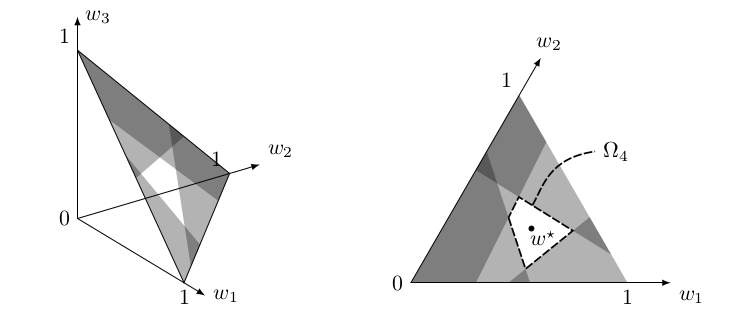
\includegraphics[width=0.75\textwidth]{referenced_promethee/src/representation_from_Eppe.png}
    \caption{Planar representation of the weight domain for a 3-criteria problem with 4 constraints. The darkness of each area is an indicator of the quantity of constraints that are violated inside that area. \cite{eppe2014adaptive}.}
    \label{fig:planar_representation_weight_domain}
\end{figure}


The domain of admissible weight factors being reduced at each iteration, the set $\Gamma$ of the rankings produced associated to this domain will generally also be reduced.

After some number $l$ of iterations, the remaining set $\Gamma_l$ will contain only rankings which are similar to the ranking which correctly represents the preferences of the decision maker.

This procedure should of course achieve these results by asking the less possible questions.
Indeed, if the decision maker has to answer too many queries, then the benefits of using a multi-criteria decision aid method vanish as he still has to be able to provide much of the information about his preferences himself.

Therefore, a particular attention is given to the choice of the queries that will be asked.
The query generation scheme used in \cite{eppe2014adaptive} is based on the idea presented by Iyengar et al. in \cite{iyengar2001evaluating}. It consists in asking queries which split the space of admissible weights the most equally possible in two (maximizing the worst case reduction of the domain).
Since the answer of the decision maker can not be anticipated, it is not known which of the two splitted parts of the domain will be eliminated by the new constraint.

The query asked at each iteration $i$ is generated as follows \cite{eppe2014adaptive}:
\begin{enumerate}
    \item The center $w^{\star}$ of the domain of admissible weights factors is computed.
    \item A ranking $R$ is established by applying \textsc{promethee ii} with $w^{\star}$ on $A$.
    \item The alternatives with the best rankings are kept. Each couple of these alternatives will be considered as a query candidate.
    \item The cut of $\Omega_i$ associated with each query candidate is evaluated and the query splitting this domain the most equally is asked to the decision maker.
\end{enumerate}

Some details of this procedure were voluntarily omitted in this synthesis which is aimed at helping to understand the underlying idea of this procedure. The interested reader can refer to \cite{eppe2014adaptive} for more details.

\subsubsection{Adaptive questioning procedure defining sets of reference profiles}

Few differences must be taken into account when trying to find sets of reference profiles instead of vectors of weights.
Indeed, in this case, when the decision maker express his preference of an alternative $a_i$ over an alternative $a_j$, then the referenced flow of $a_i$ will have to be greater than the one of $a_j$, which means that:

\begin{equation}
    \begin{split}
        \frac{1}{p}\sum\limits_{r \in \mathcal{R}}\sum\limits^k_{c=1} & w_c \cdot \left[P_c(a_i,r) - P_c(r, a_i) \right] \\
        & > \frac{1}{p}\sum\limits_{r \in \mathcal{R}}\sum\limits^k_{c=1} w_c \cdot \left[ (P_c(a_j,r) - P_c(r, a_j)\big)\right] \\
    \end{split}
\end{equation}

Due to the nonlinearity of the preference functions $P_c$, it is not possible anymore to find linear constraints on the sets of reference profiles $\mathcal{R}$.
The domain of admissible points is also not guaranteed to be convex nor connected anymore.

Therefore, the initial domain of possible sets of reference profiles will be represented by a sufficiently large set of points $S$. These points are selected uniformly at random in the $p \times k$ dimensional space representing all the possible sets of $p$ reference profiles.

At each iteration $i$, the points which are not consistent with the answer given by the decision maker will be removed from this set.
The remaining set, after  each query, will be called $S_i$.

The query generation scheme has also slightly been modified.
Query candidates have not been selected using the ranking obtained with the center of admissible points.
Indeed, since the constraints are not linear anymore and since the center is not guaranteed to be an admissible point, there does not seem to be any reasons why it should be used.
Instead, since the domain considered at each iteration consists of a finite set of points $S_i$, the ranking $R^{\star}$ which is obtained with the largest number of points will be used to select the query candidates.

%Since the domain of admissible points is not convex nor connected anymore, the center of this domain is not guaranteed to be admissible.

%The center of this set of points is therefore necessarily admissible and could lead to a ranking violating existing constraints.
%Using this center $\mathcal{R}^{\star}$ as set of reference profiles to build a \textsc{referenced promethee} ranking which will be the basis for selecting the alternatives which will form the next query does not make much sense if this ranking is violating the already existing constraints and is not in the domain $\Gamma_i$ of admissible rankings.
%Therefore, instead building a ranking with the center of the domain, the \textsc{referenced promethee} ranking which is produced by the largest number of points in $S_i$ will be selected as basis for the query candidates selection.
All the couples of pairwise successively ranked alternatives are then selected as query candidates.
The query candidate which will lead to the removal of the largest amount of points in $S_{i-1}$ (in the worst case) is proposed to the decision maker.

The procedure is synthesized in Algorithm \ref{alg:RS_questioning_procedure}.

\begin{algorithm}[H]
\setstretch{1.05}
\begin{algorithmic}[1]
    \REQUIRE $A$, $\mathcal{P}$, $w$, $p$, points\_qty, procedure\_iterations
    \STATE PII\_ranking = PrometheeII(A, $\mathcal{P}$, $w$)
    \STATE constraints = $\emptyset$
    \STATE $S_0$ = initial\_points($A$, $p$, points\_qty)
    \FOR{i = 0 \dots procedure\_iterations}
        \STATE $\Gamma_i$, commonest\_ranking = analyse($S_{i}$, PII\_ranking, A, $\mathcal{P}$, $w$)
        \STATE query = evaluate\_candidates($S_i$, commonest\_ranking, A, $\mathcal{P}$, $w$)
        \STATE constraint$_i$ = ask\_DM(query, PII\_ranking)
        \STATE constraints = constraints $\cup$ constraint$_i$
        \STATE $S_{i+1}$ = update\_points($S_i$, constraint$_i$)
        \IF{size($S_{i+1}$) < points\_qty}
            \STATE $S_{i+1}$ = $S_{i+1}$ $ \cup $ add\_points(constraints, $A$, $p$)
        \ENDIF
    \ENDFOR
\end{algorithmic}
\caption{Adaptive questioning procedure for finding a set of reference profiles}
\label{alg:RS_questioning_procedure}
\end{algorithm}

Where the following functions could require some additional information:

\begin{description}
    \item[initial\_points():] build the initial set of points. Each point represents a set of reference profiles composed of $p$ profiles. The evaluations of these initial sets of reference profiles are selected uniformly at random between ``$0.5 \times$the lowest evaluation in $A$'' and ``$1.5 \times$the highest evaluation in $A$''.
    \item[evaluate\_candidates():] computes, for each pair $a_i$ and $a_j$ of successive alternatives in the \textit{commonest\_ranking}, the minimal number of points that would be removed from $S_i$ if they formed the next query.
        This is done by computing for each point whether $a_i$ or $a_j$ would obtain the highest referenced flow.
        The pair of alternatives which maximizes the minimal number of points that could be removed is returned as the next query.
    \item[update\_points():] returns a reduced set of points by removing all points from the given set which do not respect the new constraint.
    \item[analyse(): ] analyses all the rankings produced by the remaining points to provide some information about their convergence. This is needed both to be able to analyse the performances of the procedure and to be able to decide after which iteration it should stop. \\
        In the algorithm presented here above, only the different rankings ($\Gamma_i$), and the commonest ranking  obtained from $S_i$ are computed (for readability purposes). Of course, the other indicators that will be used in the empirical results (such as the correlation coefficients between these rankings and the \textsc{promethee ii} ranking) are also computed with this function.
    \item[add\_points():] Due to performances issues, it is not possible to start with a set $S_0$ which contains enough points. Therefore, if at a given iteration, the quantity of points remaining is too low, then some points are added. The points added must of course respect it already imposed constraints.

        When several of these constraints have already been imposed, it can become difficult to find new points which satisfy all these constraints at random. To overcome this difficulty, two approaches are used simultaneously. At each iteration, the procedure tries to add some random points and the also tries to add points close to the already existing ones (by multiplying their coordinates by some factors selected uniformly at random between 0.9 and 1.1).
\end{description}

The results of the application of this algorithm on some random sets of alternatives are illustrated in the next section.

\subsubsection{Some results of the application of the adaptive questioning \\ procedure}

The questioning procedure has been applied on different data sets with contrasting results.
The study of its application on three sets of alternatives illustrating this contrast will be detailed here under.

These three sets of alternatives are all composed of 20 or 30 alternatives with weight factors and preference functions taken uniformly at random as usual.
The sets of reference profiles considered are always composed of 4 profiles.

The first results are shown in Table \ref{tbl:questioning_procedure_EPI_1} where the procedure was applied on 20 random alternatives taken from the \textsc{epi} data set.

\begin{table}[h]
    \centering
    \begin{tabular}{c c           c             c                    c               c            c          c}
        \toprule
        $i$  & $\mid S_i \mid$ & $\mid \Gamma_i \mid$ & $\tau_{min} $   & $\tau_{max}$ & $\tau_{\mu}$& $\tau_{med}$  & removed  \\
         \midrule
 5 &  3006   &  925  &-0.200 & 1.000 & 0.405 & 0.410 &  1441  \\ 
 9 &  3000   &  333  &-0.189 & 1.000 & 0.537 & 0.610 &  1387  \\ 
11 &  2384   &  130  &-0.126 & 1.000 & 0.646 & 0.715 &  1584  \\ 
13 &  2218   &  32   & 0.178 & 1.000 & 0.757 & 0.715 &  1520  \\ 
14 &  2905   &  22   & 0.421 & 1.000 & 0.916 & 1.000 &   611  \\ 
16 &  3291   &   3   & 0.705 & 1.000 & 0.996 & 1.000 &   124  \\ 
17 &  3167   &   1   & 1.000 & 1.000 & 1.000 & 1.000 &    0   \\ 
        \bottomrule
    \end{tabular}
    %\captionsetup{width=10cm}
    \caption{Adaptive questioning procedure analysis on a subset composed of 20 alternatives taken at random from the \textsc{epi} data set}
    \label{tbl:questioning_procedure_EPI_1}
\end{table}

The two first columns of the table contain the iteration number and the size of the set of admissible points (at the beginning of this iteration).
The next column contains the total number of rankings that are induced by all these points.
Then, the four next columns contain some characteristics of these rankings.
They respectively contain the minimal, the maximal, the average and the median correlation coefficient between the rankings in $\Gamma_i$ and the \textsc{promethee ii} ranking.
The last column contains the number of points that are removed due to the addition of the new constraint.

This data set is the one where the smallest number of iterations was needed in order to obtain a set of points $S$ containing only points reproducing the \textsc{promethee ii} ranking.
Still, 16 questions had to be asked to arrive at this situation.
%Still, 17 questions had to be asked to the decision maker in order to obtain a set of admissible points composed only of points that reproduces the \textsc{promethee ii} ranking.
This quantity could seem to be pretty high since $A$ is composed of only 20 alternatives.



More details about the evolution of the admissible correlation coefficients can be seen in the boxplot representation in Figure \ref{fig:boxplot_epi_seed_1}.
%Here under a boxplot representation of the correlation coefficients obtained by the admissible rankings at each iteration can be seen:

\begin{figure}[!h]
    \centering
    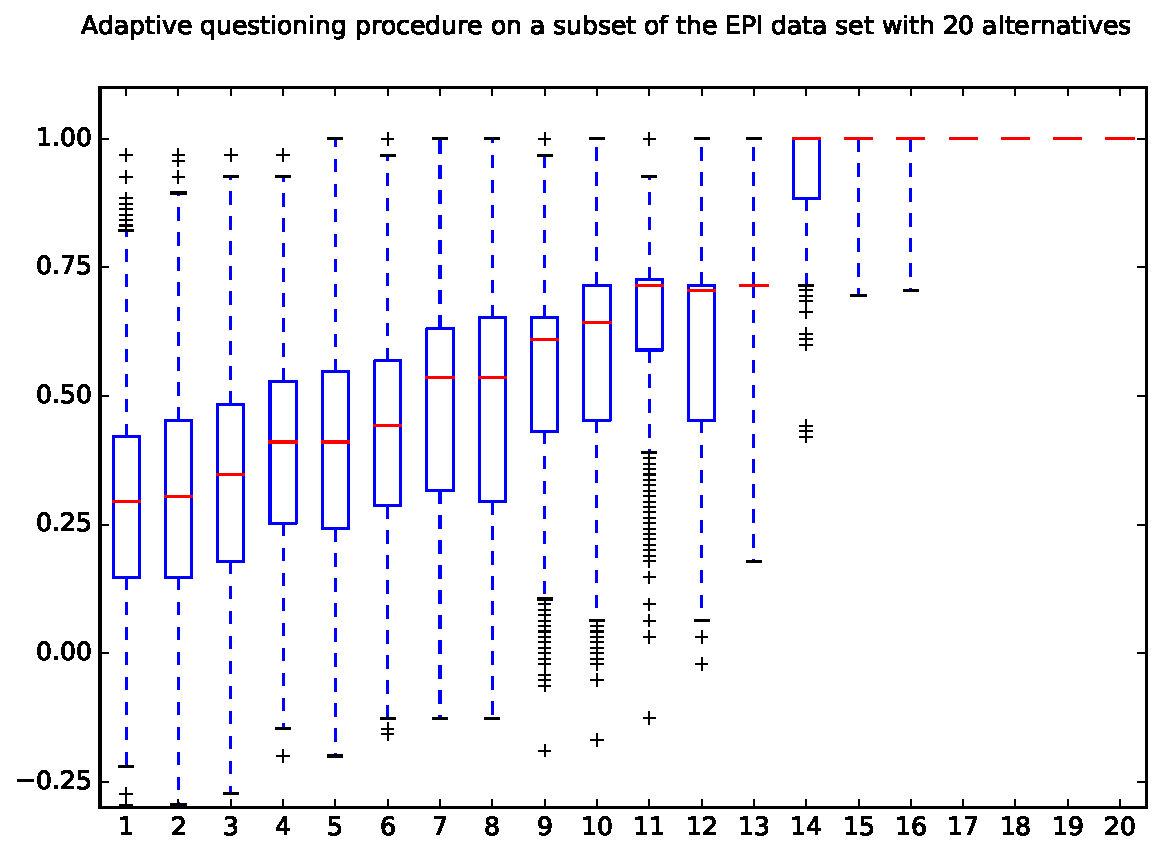
\includegraphics[width=0.9\textwidth]{referenced_promethee/src/boxplot_epi_seed_1.pdf}
    \caption{Kendall's correlation coefficient between the \textsc{promethee ii} ranking and the admissible rankings during an application of the adaptive questioning procedure on a set of 20 alternatives taken at random from the \textsc{epi} data set}
    \label{fig:boxplot_epi_seed_1}
\end{figure}

It can be seen that until the $13$th iteration of the procedure the worst correlation coefficient was still about $0.18$.
Until this iteration, the median, average and minimal correlation coefficient observe a slow but continuous growth. Then, between the 13th and 14th iteration, a sudden growth occurs.
% However, a slow but nearly continuous growth can be observed for the average and median correlation coefficients followed by a sudden growth at after the $11$th query.

\newpage
The second set of alternatives on which the results of the adaptive questioning procedure are illustrated is composed of 20 other alternatives taken again at random from the \textsc{epi} data set.

The results of this application are shown in Table \ref{tbl:questioning_procedure_EPI_0} and in the boxplot  represented in Figure \ref{fig:boxplot_epi_seed_0}.

\begin{table}[!h]
    \centering
    \begin{tabular}{c c           c             c                    c               c            c          c}
        \toprule
        $i$  & $\mid S_i \mid$ & $\mid \Gamma_i \mid$ & $\tau_{min} $   & $\tau_{max}$ & $\tau_{\mu}$& $\tau_{med}$  & points removed  \\
         \midrule

 5 &  3235   &  851  &-0.052 & 1.000 & 0.616 & 0.610 &  1544\\   
 8 &  3000   &  272  & 0.126 & 1.000 & 0.791 & 0.810 &  1363 \\  
12 &  2248   &  112  &-0.031 & 1.000 & 0.878 & 0.989 &   376  \\ 
13 &  3061   &  73   & 0.178 & 1.000 & 0.886 & 1.000 &   483  \\ 
16 &  2438   &  21   & 0.452 & 1.000 & 0.956 & 1.000 &   171  \\ 
20 &  2465   &   1   & 1.000 & 1.000 & 1.000 & 1.000 &     \\ 
        \bottomrule
    \end{tabular}
    %\captionsetup{width=10cm}
    \caption{Adaptive questioning procedure analysis on a subset composed of 20 alternatives taken at random from the \textsc{epi} data set}
    \label{tbl:questioning_procedure_EPI_0}
\end{table}

\begin{figure}[!h]
    \centering
    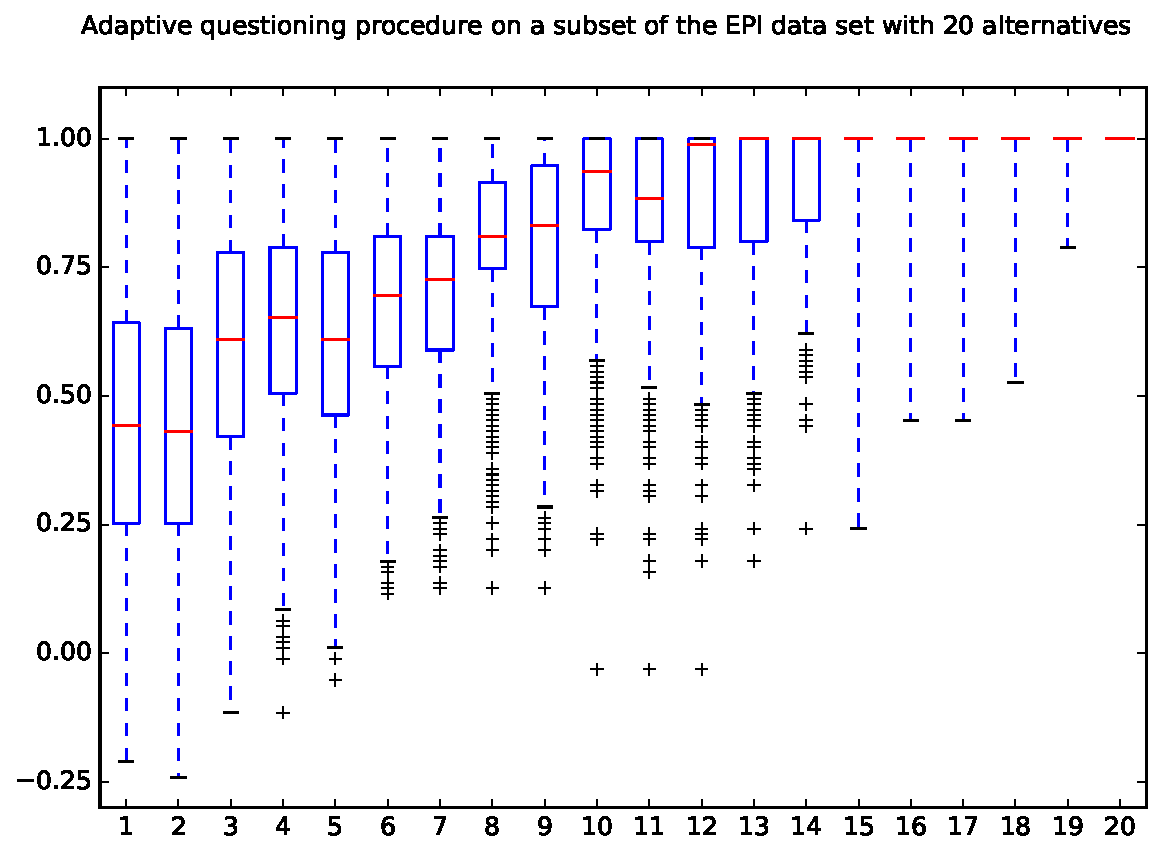
\includegraphics[width=0.88\textwidth]{referenced_promethee/src/boxplot_epi_seed_0.pdf}
    \caption{Kendall's correlation coefficient between the \textsc{promethee ii} ranking and the admissible rankings during an application of the adaptive questioning procedure on a set of 20 alternatives taken at random from the \textsc{epi} data set}
    \label{fig:boxplot_epi_seed_0}
\end{figure}

For this set of alternatives, a larger number of queries had to be asked in order to reduce the set to only points reproducing the \textsc{promethee ii} ranking, and the worst admissible correlation tau stays very low until the $18$th query. On the other hand, the median and average correlation coefficient grow faster.


The last set of alternatives on which the procedure is illustrated is a set of 30 alternatives taken at random from the \textsc{geq} data set.

Again, the results of this application can be seen in the table and in the boxplot hereunder.

\begin{table}[h]
    \centering
    \begin{tabular}{c c           c             c                    c               c            c          c}
        \toprule
        $i$  & $\mid S_i \mid$ & $\mid \Gamma_i \mid$ & $\tau_{min} $   & $\tau_{max}$ & $\tau_{\mu}$& $\tau_{med}$  & points removed  \\
         \midrule
 5 &  3010   & 2752  &-0.195 & 0.783 & 0.291 & 0.296 &  1451  \\ 
10 &  2495   & 1935  &-0.043 & 0.797 & 0.357 & 0.351 &  1159  \\ 
15 &  2019   & 1146  & 0.080 & 0.857 & 0.415 & 0.402 &   947  \\ 
20 &  2095   & 1042  & 0.075 & 0.935 & 0.456 & 0.420 &  1056  \\ 
25 &  2204   &  131  & 0.425 & 0.848 & 0.672 & 0.668 &   985  \\ 
30 &   931   &  79   & 0.356 & 0.935 & 0.728 & 0.728 &      \\ 
        \bottomrule
    \end{tabular}
    %\captionsetup{width=10cm}
    \caption{Adaptive questioning procedure analysis on a subset composed of 30 alternatives taken at random from the \textsc{geq} data set}
    \label{tbl:questioning_procedure_GEQ_3}
\end{table}

\begin{figure}[!h]
    \centering
    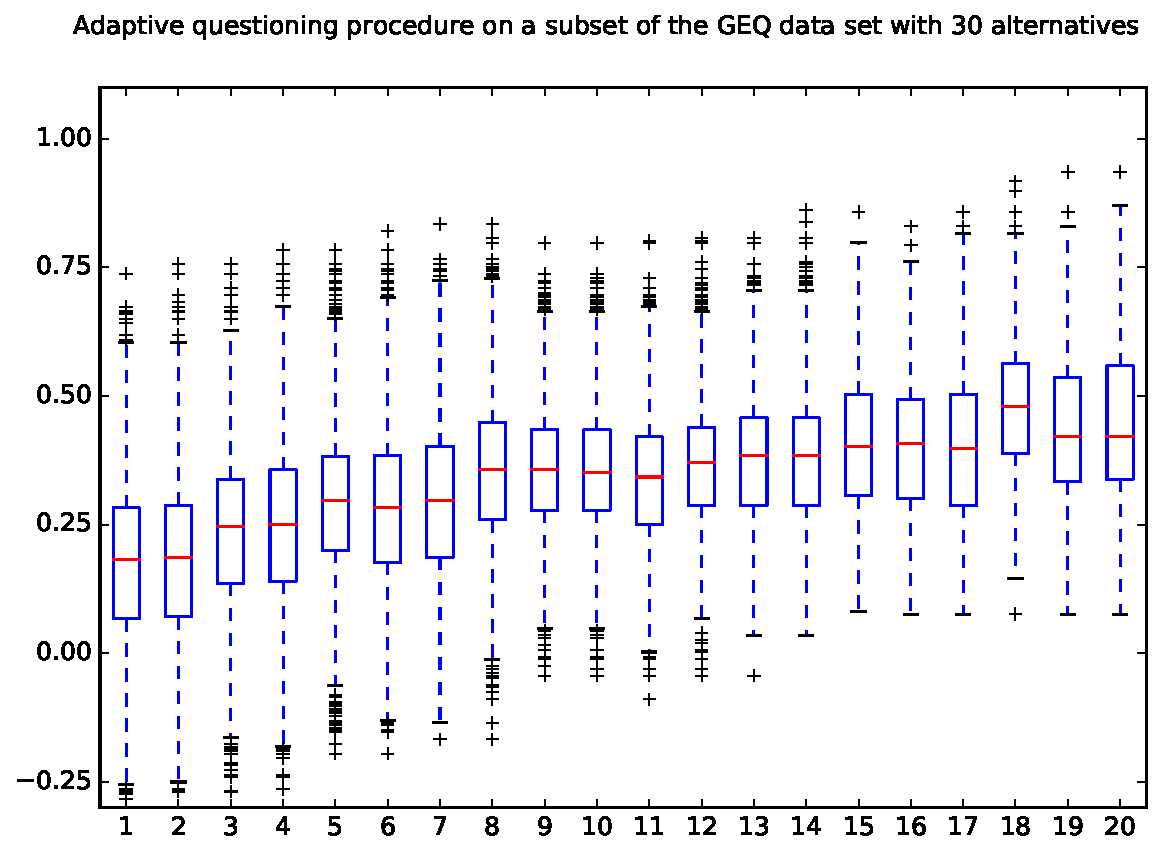
\includegraphics[width=0.85\textwidth]{referenced_promethee/src/boxplot_geq_seed_3.pdf}
    \caption{Kendall's correlation coefficient between the \textsc{promethee ii} ranking and the admissible rankings during an application of the adaptive questioning procedure on a set of 30 alternatives taken at random from the \textsc{geq} data set}
    \label{fig:boxplot_geq_seed_3}
\end{figure}

This set of alternatives is one of the set of alternatives for which the genetic algorithm presented in section \ref{sec:genetic_alg} could not find any set composed of 4 reference profiles reproducing the \textsc{promethee ii} ranking.
It is therefore not surprising that the questioning procedure does not succeed at finding one neither.

The correlation coefficients for this application of the procedure do not grow very much. As shown in the Figure \ref{fig:boxplot_geq_seed_3}, the median correlation coefficient does nearly not grows during the 20 first iterations. During the 10 next iteration however, the average and median coefficients grow faster but stay under $0.73$.
It can also be noted that at the beginning of the 30th iteration, the set of admissible points was only composed of 900 points. This is due to the difficulty of the procedure to find new points when some constraints have already been imposed.

The results of the adaptive query procedure applied on these three different data sets are not encouraging.
In the best case, about 10 questions were needed to obtain a set of points whose ``average'' ranking is similar enough to the \textsc{promethee ii} ranking (when the method is applied on a set of 20 alternatives).
In the worst case, it can happen that this procedure does not converge to a set of points which produce only rankings similar to the \textsc{promethee ii} method. We can therefore conclude that the procedure is failing in some cases.

However, this procedure has been useful as it produced a lot of points (which, it should not be forgotten, represent sets of reference profiles) which lead to \textsc{referenced promethee} rankings equal to the \textsc{promethee ii} ones.
These sets of reference profiles will briefly be analysed in the next section in order to try to find some possible characterisations of these sets.
Such characterisations could be helpful to increase the understanding of the relations between sets of alternatives and the efficiency of strategies used to build set of reference profiles, or eventually to try to imagine new strategies.

\subsection{Analysis of the satisfactory sets of reference profiles found}

Different sets of reference profiles producing a \textsc{referenced promethee} ranking identical to the \textsc{promethee ii} one were found.
These sets of reference profiles have been analysed in order to try to find some similarities which could lead to some indications about how to build such sets of reference profiles.

For instance, the table hereunder shows the expectation of the ratio between the variance of the reference profiles over the variance of the set of alternatives for three different decision problems with alternatives taken from the \textsc{shanghai} data set:

\begin{equation}
    E_c = E[\frac{D^2(f_c(r))}{D^2(f_c(a_i))}]  \qquad r \in \mathcal{R}, a_i \in A
    \label{eq:expectation_ratio_var}
\end{equation}


\begin{table}[h]
    \centering
    \begin{tabular}{L @{\hskip 0.75cm} R R R R R R}
        \toprule
        A_i   & E_1 & E_2  & E_3& E_4& E_5& E_6 \\
        \midrule
        A_1 & 4.0   & 4.3   & 4.7   & 4.3   & 2.0   & 2.5   \\
        A_2 & 5.9   & 2.9   & 7.2   & 7.2   & 4.7   & 2.5   \\
        A_3 & 4.1   & 4.2   & 2.2   & 1.7   & 2.5   & 3.9   \\
        \bottomrule
    \end{tabular}
    %\captionsetup{width=10cm}
    \caption{Expectations of the ratio between the variance of the set of reference profiles and the set of alternatives for sets of reference profiles which reproduce the \textsc{promethee ii} ranking exactly.}
    \label{tbl:E_sigma}
\end{table}

We can deduce from this table that the variance of the evaluations of the sets of reference profiles should be higher than the one of the sets of alternatives.
However, of how much this variance must be higher is not clear.
Indeed, these variances vary significantly from one criterion to another and from one set of alternatives to another.
The same observations have been done for sets of alternatives taken from the \textsc{epi} and \textsc{geq} data sets.

Some other estimators have been studied such as, for instance, the expectation of the ratio between the mean of the evaluations of the reference profiles and the mean of the evaluations of the alternatives.
These studies did not lead to any interesting property and are therefore not shown.

Different sets of reference profiles reproducing the \textsc{promethee ii} ranking for a same set of alternatives (with the same decision maker) can be represented in a parallel coordinates plot.

A typical parallel coordinate boxplot obtained by plotting two sets of reference profiles is shown in Figure \ref{fig:parallel_coordinate_sha}.

\begin{figure}[h]
\centering
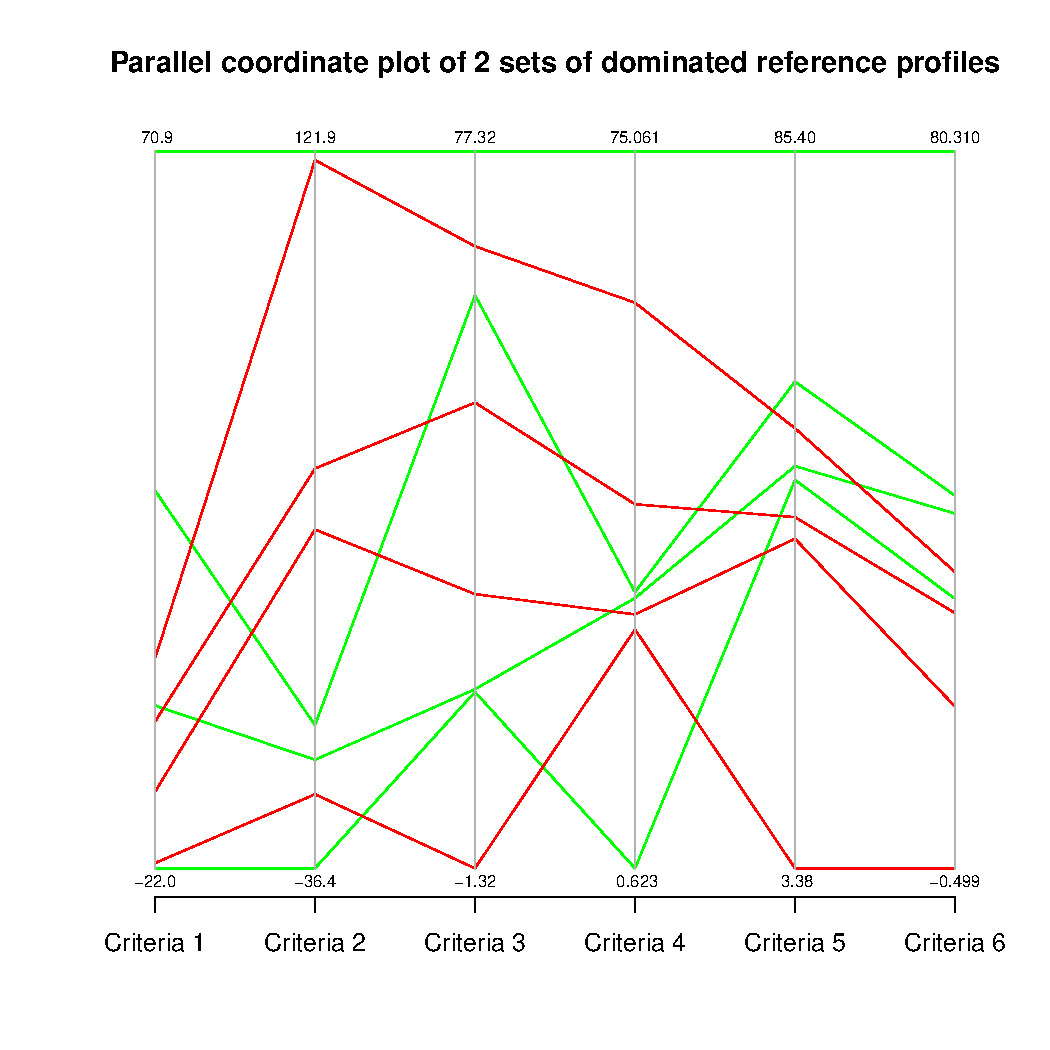
\includegraphics[width=\textwidth]{referenced_promethee/src/parallel_coordinate_plot_sha_seed_0_RS_1_2.pdf}
    \caption{Parallel coordinate plot of two sets of reference profiles reproducing the \textsc{promethee ii} ranking for a subset of alternatives taken at random from the \textsc{shanghai} data set.}
    \label{fig:parallel_coordinate_sha}
\end{figure}

Once again, no particular characteristic has been found during the study of these parallel coordinates plots. The profiles taken from different sets do not seem to have any similarities.

\section{Conclusions and synthesis of the \\ \textsc{referenced promethee} method}

\textsc{referenced promethee} does not suffer from the rank reversal phenomenon.
However, it produces rankings strongly dependent on the set of reference profiles used.

It has been seen that there generally exist some sets of reference profiles which lead to the same or highly similar rankings as \textsc{promethee ii}, which are considered to be satisfying rankings.

\newpage
However, no method was found that was able to build such sets for any decision problems (without using the corresponding \textsc{promethee ii} ranking).
The procedures based on the strategies and on the adaptive questioning procedure (sections \ref{sec:strategies} and \ref{sec:questioning_procedure}) both produce rankings which similarities with the \textsc{promethee ii} ones strongly depend on the set of alternatives and on the decision maker.
These rankings are in some cases not similar enough to the \textsc{promethee ii} ranking to be considered as satisfying.



